% !TEX root = ../main.tex
%

\chapter{L-curve}

\index{L-curve}
ここでは正則化パラメータを決める手法の1つである
L-curve法について説明する.

\begin{figure}[tp]\centering
    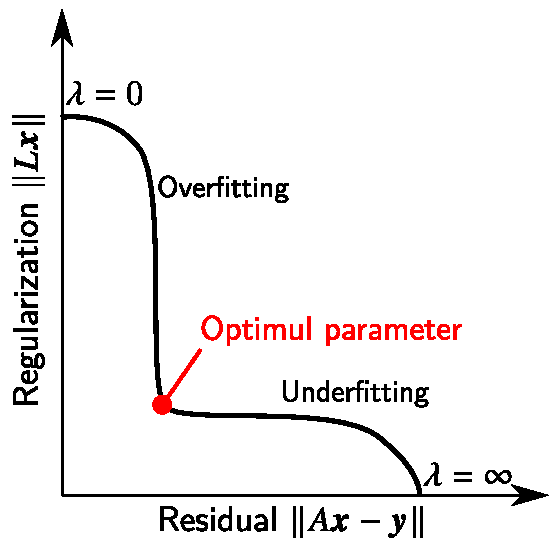
\includegraphics{./regularization/L-curve.pdf}
    \caption{L-curve の概形}
    \label{fig:regularization_l-curve_l-curve}
\end{figure}

正則化の式 \eqref{eq:regularization_intro_general-regularization} を最小化する
$\bm{x}$ を $\bm{x}_\lambda$ として,
横軸を残差 $\|A\bm{x}_\lambda-\bm{y}\|$,
縦軸を正則化項 $R(\bm{x}_\lambda)$ とし,
正則化パラメータ $\lambda$ を変えたときの
プロットを L-curve と呼ぶ.
L-curve は一般に図 \ref{fig:regularization_l-curve_l-curve} のような L の字を
描いている場合が多い.
単純にノルムをプロットするよりも
両対数グラフにプロットする方が
後述する曲線の特徴をはっきりさせられる他,
スケールの違いによる影響を
抑えられるなどのメリットもあるという
\cite{Hansen1998}.

図 \ref{fig:regularization_l-curve_l-curve} のように L-curve が得られた場合,
L の字の曲がり角にあたる赤い点の部分から左上の方では
残差がほとんど減らずに正則化項が増加しており,
右下の方では正則化項がほとんど減らずに残差が増えているため,
両方のバランスが取れている L の字の曲がり角を取るのが良いと考えられる.
そこで,L-curve の曲がり角を数値的に求める手法について考える.

ここでは,文献 \cite{Hansen1998} に従い次の関数の組を考える.
\begin{equation}
    (\xi(\lambda), \eta(\lambda))
    =(\log\|A \bm{x}_\lambda - \bm{y}\|, \log{R(\bm{x})})
\end{equation}
L-curve の曲がり角は曲線 $(\xi(\lambda), \eta(\lambda))$ の
曲率が最も大きい部分と考えられるため,曲率
\begin{equation}
    \kappa(\lambda) =
    \frac{\xi'\eta'' - \xi''\eta'}
    {\left( (\xi')^2 + (\eta')^2 \right)^{3/2}}
    \label{eq:regularization_l-curve_curvature}
\end{equation}
を求め,それを最大化する.
曲率が何らかの手法で求まれば,
1 変数の最適化については
\ref{chap:opt_one-dim-section-search} 章で説明しているため,
ここでは曲率の計算法について考える.

\section{Tikhonov 正則化の場合}

Tikhonov 正則化(\ref{chap:regularization_tikhonov} 章)の場合,
式 \eqref{eq:regularization_l-curve_curvature} にある各種微分を
陽的に表すことができる
\cite{Hansen1992,Mueller2012}.

\begin{align}
    \frac{d}{d\lambda} \|A \bm{x}_\lambda - \bm{y}\|_2^2
     & = \sum_{i=1}^r \frac{2 \lambda \sigma_i^2}{(\sigma_i^2 + \lambda)^3}
    \left(\bm{u}_i^* \bm{y}\right)^2
    \\
    \frac{d}{d\lambda} \|\bm{x}_\lambda\|_2^2
     & = \sum_{i=1}^r \frac{-2 \sigma_i^2}{(\sigma_i^2 + \lambda)^3}
    \left(\bm{u}_i^* \bm{y}\right)^2
    \\
    \frac{d^2}{d\lambda^2} \|A \bm{x}_\lambda - \bm{y}\|_2^2
     & = \sum_{i=1}^r \frac{2 \sigma_i^4 - 4 \lambda \sigma_i^2}
    {(\sigma_i^2 + \lambda)^4}
    \left(\bm{u}_i^* \bm{y}\right)^2
    \\
    \frac{d^2}{d\lambda^2} \|\bm{x}_\lambda\|_2^2
     & = \sum_{i=1}^r \frac{6 \sigma_i^2}{(\sigma_i^2 + \lambda)^4}
    \left(\bm{u}_i^* \bm{y}\right)^2
\end{align}

これらは式
\eqref{eq:regularization_tikhonov_residual-by-svd},
\eqref{eq:regularization_tikhonov_regularization-term-by-svd}
から求めることができる.

\section{一般の場合}

前節のように残差項と正則化項の微分を解析的に計算できれば簡単に曲率の計算ができるが,
必ずしも正則化項を簡単に計算できるとは限らない.
$\xi(\lambda)$ と $\eta(\lambda)$
の微分を解析的に計算できない場合は,
サンプル点に対する 3 次の自然スプラインによる補間を用いて L-curve の曲率を計算できる.
ただし,このときは $(\xi(\lambda),\eta(\lambda))$ を
$\lambda$ の関数として補間するのではなく,
$(\lambda(t), \xi(\lambda(t)), \eta(\lambda(t)))$
のような媒介変数 $t$ を用いた
3 次元データを補間しなければ上手くいかない
\cite{Hansen1998,Hansen1993}
\footnote{例えば,サンプル点の距離を用いて長さのパラメータを作り,それを $t$ にすることが考えられる.}.
また,スプラインの計算において
$(\xi(\lambda(t)), \eta(\lambda(t)))$
の近いサンプル点があると
最終的な曲率に影響が出る場合があるため,
そのような点を省いて計算を行う必要がある.
